% v2-acmsmall-sample.tex, dated March 6 2012
% This is a sample file for ACM small trim journals
%
% Compilation using 'acmsmall.cls' - version 1.3 (March 2012), Aptara Inc.
% (c) 2010 Association for Computing Machinery (ACM)
%
% Questions/Suggestions/Feedback should be addressed to => "acmtexsupport@aptaracorp.com".
% Users can also go through the FAQs available on the journal's submission webpage.
%
% Steps to compile: latex, bibtex, latex latex
%
% For tracking purposes => this is v1.3 - March 2012

\documentclass[prodmode,acmtecs]{acmsmall} % Aptara syntax


% JPO ADDED PACKAGES
\usepackage{epsfig}  
\usepackage{amsmath} 
\usepackage{amssymb} 
%\usepackage{amsthm}  
\usepackage{listings} 
\usepackage{color}
%\usepackage{enumerate}
\usepackage{enumitem}
\usepackage{multirow}
\usepackage{lastpage}
\usepackage{geometry}
\usepackage{fancyhdr}
\usepackage[all]{xy}
\usepackage{wrapfig}
\usepackage{listings}
\usepackage{url}
\usepackage{tikz}
\usepackage{graphicx}
%\usepackage{caption}
%\usepackage{subcaption}
\usepackage[justification=centering]{caption}
\usetikzlibrary{arrows}
\lstset{language=C, tabsize=4, basicstyle=\ttfamily}

% JPO COMMANDS
\newcommand\etal{\emph{et al.}}
\newcommand{\jp}[1]{[{\emph{\textcolor{blue}{JP: #1}}}]}
\newcommand{\mg}[1]{[{\emph{\textcolor{red}{MG: #1}}}]}

% Package to generate and customize Algorithm as per ACM style
\usepackage[ruled]{algorithm2e}
\renewcommand{\algorithmcfname}{ALGORITHM}
\SetAlFnt{\small}
\SetAlCapFnt{\small}
\SetAlCapNameFnt{\small}
\SetAlCapHSkip{0pt}
\IncMargin{-\parindent}

% Metadata Information
\acmVolume{42}
\acmNumber{42}
\acmArticle{42}
\acmYear{2014}
\acmMonth{42}

% Document starts
\begin{document}

% Page heads
\markboth{M. Gerrand and J.P. Ore}{On Spatial Abstractions from Trace Data}

% Title portion
\title{On Spatial Abstractions from Trace Data}
\author{MITCH GERRARD
\affil{University of Nebraska}
JOHN-PAUL ORE
\affil{University of Nebraska}}
% NOTE! Affiliations placed here should be for the institution where the
%       BULK of the research was done. If the author has gone to a new
%       institution, before publication, the (above) affiliation should NOT be changed.
%       The authors 'current' address may be given in the "Author's addresses:" block (below).
%       So for example, Mr. Abdelzaher, the bulk of the research was done at UIUC, and he is
%       currently affiliated with NASA.

\begin{abstract}
The abstract goes here, usually written last.
\end{abstract}

\category{I.2.4}{Knowledge Representation Formalisms and Methods}{Representations (procedural and rule-based}

\terms{Design, Algorithms}

\keywords{Spatial Abstraction, Knowledge Representation}

\acmformat{Mitch Gerrard, John-Paul Ore, 2014. On Spatial Abstractions from Trace Data.}
\begin{bottomstuff}

%This work is supported by the National Science Foundation, under
%grant CNS-0435060, grant CCR-0325197 and grant EN-CS-0329609.

Author's addresses: M. Gerrard and J.P. Ore, Computer Science and Engineering,
University of Nebraska
Lincoln, Nebraska, 68588. 
\end{bottomstuff}

\maketitle



\section{Introduction}

The world is full of moving things, and increasingly, things know where they are. 
Ubiquitous sensor technologies, like GPS, combined with networked storage enables us to continually detect and archive spatial movement.
These myriad data points can answer questions of great value, including geospatial distributions, trends and traffic flows, popular restaurants, migration patterns and much more.

\begin{wrapfigure}{l}{0.42\textwidth}
  \centering
  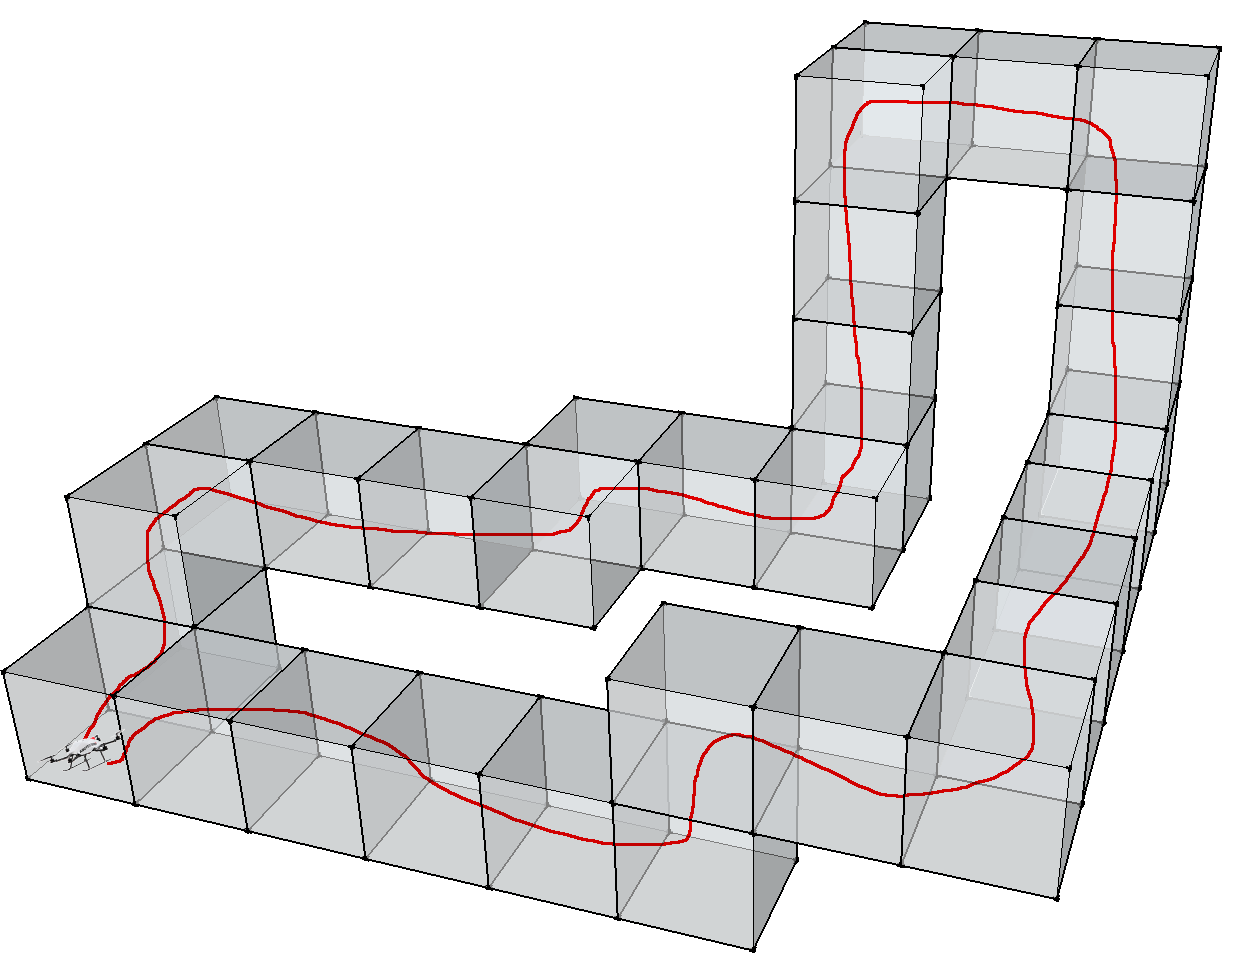
\includegraphics[width=0.42\textwidth]{./figures/path_overview}
  \caption{Unit cube space used in spatial abstraction.}
  \label{fig:unitCubes}
\end{wrapfigure}

However, we can be overwhelmed because we are ``drowning in data"~\cite{morse1993drowning}.
Further, it can be difficult to examine high-level relationships because points and lines are specific; the story is at the level of the forest and we can only see the trees.  
Often it is only feasible to analyze large data sets by choosing an appropriate level of abstraction.
The work presented here is about one such kind of abstraction.
We consider a ``spatial abstraction" where particular points in space-time are mapped to unit cubes, as shown in Fig.~\ref{fig:unitCubes}.
Using techniques inspired by software analysis, specifically Daikon invariants~\cite{kataoka2001automated}, we use trace data gathered as an object moves and explore the properties of movement of things at a higher level.

In this paper, we set forth our technique for abstracting away from particular points, 
implement our technique in a prototype tool, ``FuzzyCubicCrumbTeleportation", 
collect real movement data from a small flying robot, 
and validate our tool's ability to detect spatial properties on one or more actors.

The paper is organized as follows:
Section~\ref{sec:background} gives an overview of both spatial analysis and the Daikon invariants analysis tool;
Section~\ref{sec:technique} describes the method of spatial abstraction, including defining terms and a table of formalized properties;
Section~\ref{sec:tool} provides an overview of our tool that implements this method of analysis;
Section~\ref{sec:application} shows an initial application of our tool to a real robotic system;
Section~\ref{sec:related} situates this work relative to other kinds of movement analysis;
in section~\ref{sec:observations} we reflect on some unexpected and unexplored features of spatial abstraction;
and finally, section~\ref{sec:conclusion} summarizes this work and describes future lines of inquiry. 





\section{Background}
\label{sec:background}

Many people conceive of space in the manner of Descartes, where a fixed world frame with three perpendicular axes identify an exact position at any point.  
Yet more sophisticated observers follow Minkovsky~\cite{minkowski1952space} and imagine curvature in space time.
We're interested in a coarsening of these perspectives, imaging the universe cut into regular stacks of identical boxes, akin to an occupancy grid~\cite{moravec1985high}, or to use more technical terms, a tessellation of \rthree by a unit cuboid.

%For example, given a world frame centered directly under your feet, a point in your thumb might be described as $p_{thumb} = (x,y,z) = (0.2m, 0.3m, 0.4m)$.
%As your thumb moves, the Cartesian coordinates describing this point take on different values over time.
%If we consider some interval, $\delta t$, the set of all positions of $p_{thumb} = P$ describes the movement of this point during $\delta t$.

%However, with real systems in the world there are at least two limitations to $P$: $P$ is a finite sequence of points, and any $p \in P$ is uncertain with a quantifiable confidence.
%Let's denote $P'$ as a finite, uncertain version of $P$.
%Because $P'$ is uncertain, we can over-approximate the set of position points of our thumb by considering a kind of box, a bounding cubic volume defined by a set of 8 points, $v = {a,b,c,d,e,f,g,h}$.
%This over-approximation is useful because we can then imagine the box moving in space and if the box never intersects with an obstacle during a movement, they we can move our thumb as we imagined and know that we won't have any collisions.

This kind of coarsening is used in robot planning to reason about collision-free trajectories, specifically, planning into the future~\cite{siegwart2011introduction}.

In this paper, we're considering a similar over-approximation, or abstraction, of the position of some \emph{actor}, the thing that moves, within space. 
The key difference is that we consider properties of spatial abstractions that happened in the past, instead of the future.
To do this, we adopt a very successful methodology from software engineering and implemented in the tool Daikon~\cite{kataoka2001automated}.
Daikon uses a record of what happened during the execution of a program, called a \emph{program trace}, to analyze high-level properties of software behavior.
We consider a \emph{spatial trace}, a finite time sequence of positions, and try to reason about higher-level properties of the movement.

%If we could record, or write down, a sequence of point 
%Increasingly, our world is full of things that know where they are in space.
%Some of these things can move in space and we created them and they move based on rules we design.


\section{Method}
\label{sec:method}

In this section, we develop our method for reasoning about movement within a coarse `unit cube' space.
We start from trace data of positions, identify how this trace data is transformed into occupied boxes as well as nodes in a graph, then discuss properties of one thing moving in space, then move to multiple things moving in space.

\subsection{Foundations and Definitions}
We begin with a trace $T$ of spatial data, containing a time sequence of $xyz$ positions.
We call the thing that is moving an \eb{actor}, designated by $\bigstar$.
Each element in trace $T$ occurs at a time $t$.
Let there exist a space $\cube^3 \equiv \mathbb{Z}^3$ called ``cube 3", and a function $f_{\cube}: \bigstar_i (x,y,z) \in \mathbb{R} \rightarrow (a,b,c) \in \mathbb{Z}$, such that:

$$f_{\cube}(x,y,z) = (\lfloor x \rfloor, \lfloor y \rfloor , \lfloor z \rfloor )$$

Let the $i$th element of the trace file be designated $\bigstar_i$, and to the position data in $\bigstar_i$ we apply $f_{\cube}$ and infer the existence of cube $\cube_i$.

$$\bigstar_i \Rightarrow (\cube_i | \cube_{xyz\in \mathbb{N}} = f_{\cube}(\bigstar_{xyz})$$ 

This maps every record in the trace file to a cube.
\eb{Simultaneously}, we create a root node $v_i$ in a graph $G = (V,E)$.
For each subsequence trace record $\bigstar_{i+1}$, we check if this position maps to the same cube, $\cube_i$, or to a new cube, $\cube_{j}.$
If a record maps to a new cube $\cube_{j}$, then we add a directed edge to $E$ from $v_i$ to $v_{j}$.  
We add a label the edge $(v_i, v_j)$ with the time $t$.
The node $v_i$ corresponds to $\cube_i$ and the node $v_{j}$ corresponds to $\cube_{j}$.
From the existence of this edge we say there is a path from $\cube_i$ to $\cube_j$ denoted $\cube_{i\rightsquigarrow j}$.  More formally,

$$ f_{\cube}(\bigstar_i) \neq f_{\cube}(\bigstar_{i+1}) \Rightarrow (v_i, v_j) \in E \equiv \cube_{i\rightsquigarrow j} $$


Now we have a way to map a sequence of positions records to a unit cube space in which we have embedded a graph.
The edges in the graph capture the timestamp for each position.
We are now ready to begin reasoning about properties.

\subsection{Properties of Single Actors}


\begin{tabular}{| p{2.8cm} | p{11.5cm} | }
\hline
PROPERTY & FORMALISM \\ \hline
Move to multiple places & $\phi_{\{multiplePlaces\}} = \exists (P(b_{home}, b_a), P(b_{home}, b_b)| b_a \neq b_a)$ \\ \hline
Returns Home & $\phi_{\{returnhome\}} = \exists P(b_{home}, b_{home})$ \\ \hline
No repetition & $\phi_{\{noRepetition\}} = \forall e(v_a, v_b), e(v_c,v_d) in E, v_b \neq v_c, v_a \neq v_d$ \\ \hline
 & \\ \hline
 & \\ \hline
 & \\ \hline
$\phi_{\{teleport\}}$ & $  \exists  p_t, p_{t+1} | \lnot Adjacent(b_{p_t}, b_{p_{t+1}})$ \\ \hline
Hot Box & $\phi_{\{hotBoxOfSizeN\}} = \exists b_i, v_i \in E | n \geq |\{e \in E | e(v_x, v_i), v_x \in E\}$ \\ \hline
\end{tabular}


\subsection{Properties of Multiple Actors}
\begin{tabular}{| p{2.8cm} | p{11.5cm} | }
\hline
PROPERTY & FORMALISM \\ \hline
 & \\ \hline
 & \\ \hline
 & \\ \hline
\end{tabular}

\subsection{The Ratio Cube}

\begin{wrapfigure}{l}{0.33\textwidth}
  \centering
  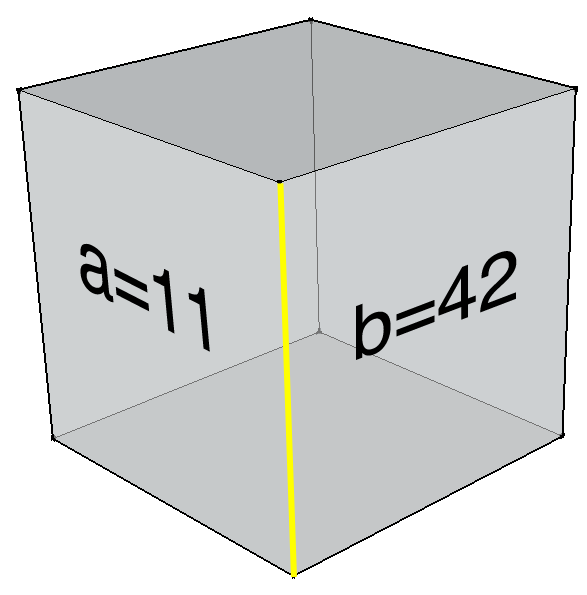
\includegraphics[width=0.32\textwidth]{./figures/counting_cube.png}
  \caption{Cube used to compare ratios of paths.  Yellow edge indicates ratio a/b.}
  \label{fig:unitCubes}
\end{wrapfigure}


Method:
\begin{itemize}
 \item partition space into boxes
 \item enumerate the boxes
 \item map a concrete positional trace through space onto its uniquely corresponding boxes
 \item sync time frames of box-traces to infer spatio-temporal properties
 \item using the spatio-temporal box-trace, derive properties (given elsewhere)
\end{itemize}

\emph{Selecting appropriate box size}

Different box sizes may generate very different properties.

\emph{Too small of a box} If you choose the boxes to be relatively small, the trace may show a teleport, which we define as a spatially disconnected box-trace.
If there are gaps of disconnected boxes, and two entities collide in the unaccounted for space, the violation of box-independence will not be inferred.

\emph{Too big of a box} If you choose the boxes to be relatively large, this may be too rough of an over approximation.
For an extreme example, an entity never registers "leaving home" if its initial box is the size of the given dimensions.
Sometimes large over-approximations are desired, such as if you only want to examine the movements across two ``hemispheres" of an entity's space.

\section{Description of Tool}
\label{sec:tool}

In this section, we describe the implementation of our tool for reasoning about spatial properties.
In the previous section, we used the language of \emph{cubes} to discuss the general methodology. 
In discussing the tool, we use the language of \emph{boxes}, \emph{box traces} and \emph{box sizes} as a way to differentiate the theory from the concrete implementation, which differ in small ways.
Our tool, written in Ruby, takes trace files, a box size, and bounding dimensions as input, and returns spatial-temporal properties inferred from the traces.  

\begin{figure}[ht]
  \centering
  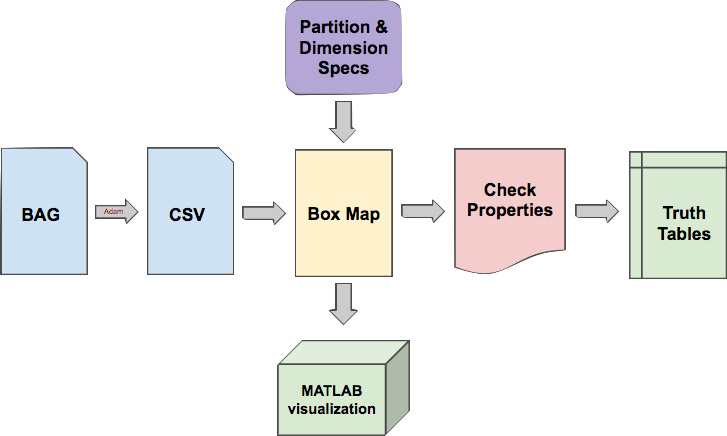
\includegraphics[width=0.95\textwidth]{./figures/workflow}
  \caption{Overview of tool workflow.}
  \label{fig:workflow}
\end{figure}

This description elaborates on the high-level workflow diagram shown in Fig.~\ref{fig:workflow}.
The trace files will be one or more .bag files.  
A bag is the file format used by the Robot Operating System (ROS) for storing ROS message data.  
Via messages, various sensors can write their values to these bags during an execution. 
These values may be examined after any run.
In our current implementation, we are only considering the values of time stamps and x, y, and z positions.

We first convert the .bag files to .csv files with four columns which contain a timestamp and the associated x, y, and z position values (in meters).  
 Our tool currently makes the assumption that we receive one \emph{complete} trace of some run, so we are not stitching together partitions of lengthy runs; this may need to be done in the future.
 Each time frame is mapped to some box, so to temporally sync the runs, we are considering the start of the run to be the global time frame of the greatest initial time frame of all given traces.

The box size is given as a single positive floating-point integer (will be a cubic box), representing the desired length of the box edges in meters.
The bounding dimensions are given as a 3-tuple of positive floating-point integers, representing the bounds of the space in which the actors move.
Given the box size, we map the position of each time frame of a single trace to the box which corresponds to an actor's position in \rthree.
 This produces a total ordering of abstracted trace positions given as a succession of boxes, which we will call a box-trace.
 
% Additionally, you need to set a flag to indicate if the input deals with a single actor or multiple actors.
 
% Based on a set of box-traces, we will check if certain properties hold.
% For example, if a trace starts out in "box 3," moves to other boxes, and occupies "box 3" at a later time, then the return home property would be set to true.
 
 The output will be a single truth table corresponding to the property you wish to check.
 %The format of these truth tables is also discussed in methods.
 You may optionally output a 3D visualization of the box-trace, displayed in MATLAB.
 
 If we are considering a single actor, given $m$ properties, the truth table will just be one row with $m$ columns containing the truth value of the corresponding property.
 If we are considering $n$ multiple actors, the output will be a truth table given as a $1 \times n$ or $n \times n$ matrix, depending on the property considered.
 For example, the returns home property only depends on a single actor, not their interactions, so the table will be a $1 \times n$ matrix with the truth value of each actor.
 But a property like box-independence considers interactions between all the actors, and so its truth table will be a $n \times n$ matrix with the truth value for box-independence between $(box_i,box_j)$ for all $1 \leq i,j \leq n$.
 
  For many of the above properties, it will be important to know specific details of violated properties (which box, which time frame, etc.); these details are being stored but we are currently only outputting binary truth values.
  
  Our tool does not yet derive a directed multigraph from the traces; this will be done in the coming weeks.
  The tool currently detects a subset of the properties mentioned in the previous section, some of which are dependent on examining a multigraph.  
\section{Experiments}

\section{Related Work}
\label{sec:related}

Our work is inspired by a software invariant analysis technique developed in the Ph.D thesis of Ernst~\cite{ernst2000dynamically} that became the tool Daikon~\cite{ernst2007daikon}.
Daikon takes as input a trace of variable values and then outputs properties (``invariants") about the values seen in that trace.
Likewise, our method takes as input spatial traces and outputs properties observed during those traces.
Unlike Daikon, which first instruments source code to generate traces, our method assumes that spatial traces are already generated by some logging mechanism of the system, in our case, ROS, the Robot Operating System~\cite{quigley2009ros}.
We are re-purposing the ideas of Daikon, as has previously been done in hardware error detection~\cite{sahoo2008using}.

In the robotics domain, using unit cubes to reason about spaces dates back at least as far as Moravec and Elfes's occupancy grids~\cite{moravec1985high}.
Their unit space denotes the existence of map obstacles detected by sonar, and this approach became a canonical approach to planning and obstacle avoidance~\cite{siegwart2011introduction,elfes1989using,borenstein1989real}.
We likewise partition spaces into coarser, regular volumes with simple occupancy properties, but additionally we embed a graph to track movement.
Occupancy grids have recently been refined by the efficient OctoMap~\cite{wurm2010octomap}.
We hope to leverage OctoMap in future applications in large spaces with multiple scales.
Unlike all known previous work with unit cubes, we reason about abstract properties of past movements rather than planning into the future.

We chose unit cubes because they are easy to work with and span \rthree. 
In 1885, Fedorov~\cite{fedorov1885elements} showed that there are exactly five ways to tessellate \rthree, and we examined the other shapes but decided that none offers advantages outweighing the ease of working with the unit cube.
Further, only the unit cube can be extended to arbitrarily high dimensions.

Blank~\etal~ use video to trace human `space-time shapes' and then identify actions based on the shapes~\cite{blank2005actions}.
We likewise consider the space occupied by an object as is moves through space, but whereas Blank~\etal~ examine a highly-detailed image with individual moving parts as inferred by pixel changes, and the speeds of those parts, we consider an object to be a point in space occupying a box.

Another approach to spatial abstraction, not involving cube spaces, is explained by Shahar and Molina~\cite{shahar1998knowledge}, who studied the properties of car traffic flow in a two-dimensional plane.
They were interested in examining the properties of groups of cars in congestion by modeling the transition from fluid-like behavior to solid behavior.
Like their work, we are coarsening space and examining properties of objects abstractly.
Unlike their approach we work in unit space and search for properties of both individual actors as well as groups.

Gatalsky~\etal~applied space-time-cube visualizations to map a trace of movement over time to a three-dimensional cube~\cite{gatalsky2004interactive}.
Like this work we are tracing movement over time, but unlike this work we reasoning about abstract properties and our main purpose is not visualization, but properties of movement.



\section{Conclusion}
\label{sec:conclusion}

This work presents a novel technique for reasoning about movement \emph{ex post facto}.
We coarsen $x,y,z$ position data to a unit cube space akin to occupancy grids.
Within this space, we identify properties of movement for individuals and groups, as well as properties of paths.
We implement this technique in a tool, and show examples of the tool's output as it identifies properties from real world position trace files.
This work demonstrates the potential of this kind of spatial abstraction for finding useful properties of moving things.

In future work, we would like to explore properties of a host of actors (swarms), apply more efficient representations of cube space such as OctoMaps, and explore the extension of these techniques to software memory shapes.






% Acknowledgments
\begin{acks}
  The authors would like to thank Dr. Matthew Dwyer and Dr. Sebastian Elbaum for there insightful feedback and scintillating conversations.
\end{acks}

% Bibliography
\bibliographystyle{ACM-Reference-Format-Journals}
\bibliography{refs}

% History dates
%\received{February 2007}{March 2009}{June 2009}




\end{document}
% End of v2-acmsmall-sample.tex (March 2012) - Gerry Murray, ACM


